\section{Окружение для тестирования и экспериментальное исследование}
В данной главе описывается реализация окружения для тестирования производительности операции композиции на символьных конечных преобразователях в библиотеке Microsoft.Automata и конечных преобразователях в YaccConstructor. Также приведено описание процесса тестирования и сделаны выводы о применимости символьных преобразователей из библиотеки Microsoft.Automata в исследовательском проекте YaccConstructor.

При изучении возможностей библиотеки, проведенном в рамках обзора, было установлено, что полная интеграция проекта YaccConstructor  и библиотеки Microsoft.Automata затруднительна. По этой причине для оценки производительности библиотеки Microsoft.Automata было необходимо создать окружение для тестирования, обеспечивающее возможность генерации тестов по одинаковым данным для разнородных сред: инструмента YaccConstructor и библиотеки Microsoft.Automata.

\subsection{Окружение для тестирования}
Предложенная архитектура среды для тестирования изображена на рис.~\ref{fig:toolStructure}, цветом обозначены модули, добавленные или модифицированные в рамках данной работы. 
\begin{figure}[h!]
    \begin{center}
        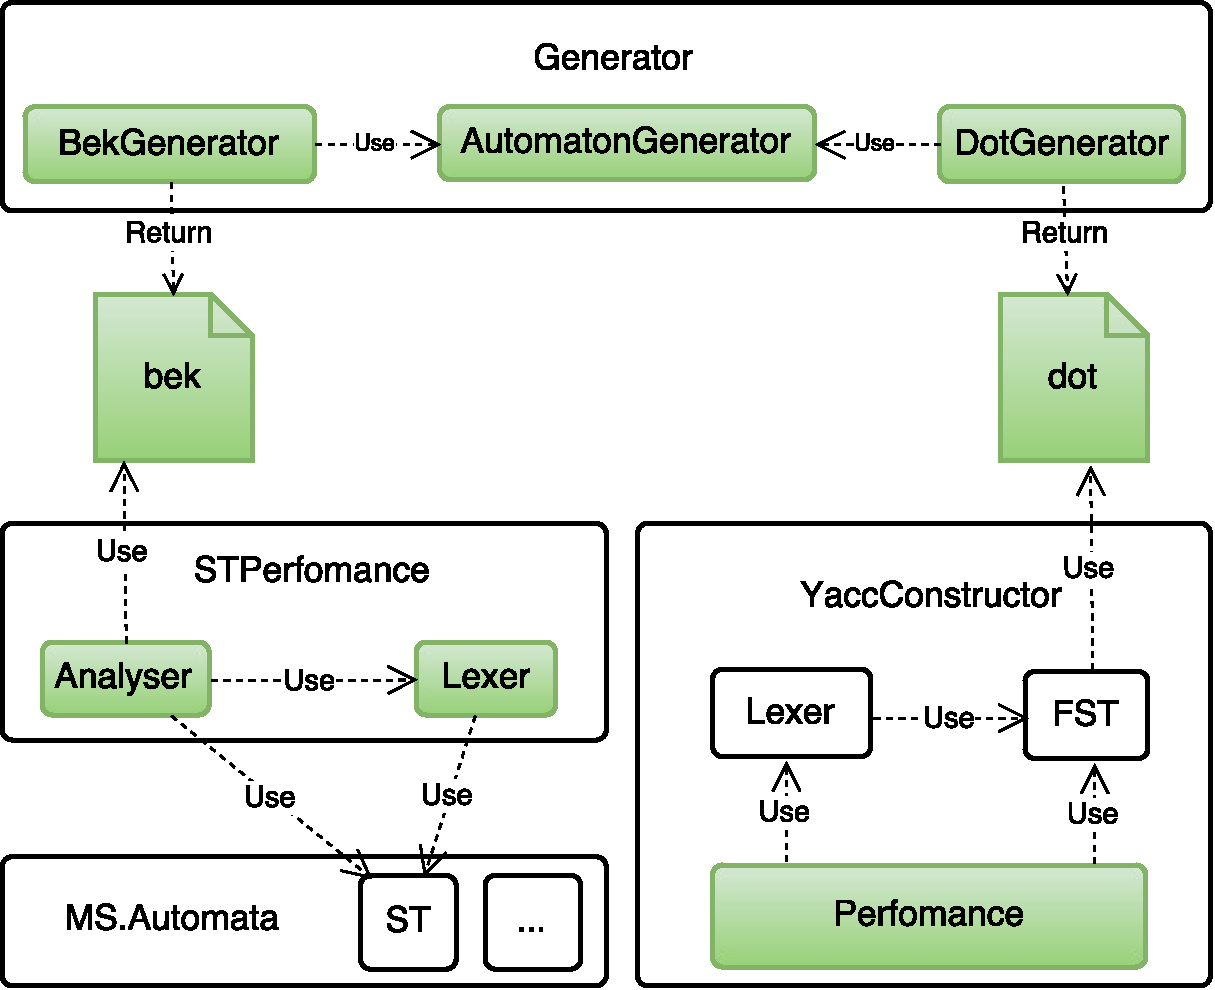
\includegraphics[width=\linewidth]{Gumin/pictures/YC.pdf}
        \caption{Архитектура среды для тестирования}
        \label{fig:toolStructure} 
    \end{center}
\end{figure}

% * <colored.lime@gmail.com> 16:40:16 25 May 2016 UTC+0300:
% косяк с графоном
Окружение состоит из:
\begin{itemize}
\item генератора конечных автоматов для создания на их основе эквивалентных преобразователей для инструмента YaccConstructor и библиотеки Microsoft.Automata;
\item генератора конечных преобразователей;
\item генератора символьных конечных преобразователей;
\item лексического анализатора в форме конечного преобразователя;
\item лексического анализатора в форме символьного конечного преобразователя;
\item модуля для анализа производительности операции композиции в проекте YaccConstructor;
\item модуля для анализа производительности операции композиции в библиотеке Microsoft.Automata.
\end{itemize}
Подробное описание компонентов приведено далее.

\subsection{Лексический анализатор}
Для сравнения времени работы операции композиции на символьных конечных преобразователях и конечных преобразователях было решено реализовать лексический анализатор арифметических выражений, аналогичный анализатору, который уже был интегрирован в проект YaccConstructor, так как язык арифметических выражений является достаточно показательным примером и включается практически в любой язык программирования.  Лексический анализатор может быть представлен в виде символьного конечного преобразователя и используется для анализа производительности библиотеки Microsoft.Automata. Реализация данного лексического анализатора выполнена на языке Bek.

\subsection{Генераторы преобразователей}
Генератор конечных автоматов (обозначен как AutomatonGenerator на рис.~\ref{fig:toolStructure}) генерирует случайные конечные автоматы с указанным количеством дуг и вершин. Результат его работы --- файл с промежуточным представлением конечного автомата, который далее интерпретируется генераторами конечных преобразователей (обозначены как BekGenerator и DotGenerator на рис.~\ref{fig:toolStructure}), которые на его основе строят программы, представляющие эквивалентные преобразователи, записанные на языках Bek и DOT соответственно. 

\subsection{Тестирование производительности композиции в проекте YaccConstructor на конечных преобразователях}
За тестирование производительности операции композиции на конечных преобразователях в проекте YaccConstructor отвечает модуль AbstractLexer.Interpreter.Perfomance (обозначен как Perfomance на рис.~\ref{fig:toolStructure}). По dot-файлам лексического анализатора арифметических выражений и dot-файлам, сгенерированными модулем DotGenerator строятся конечные преобразователи. Затем производится композиция преобразователя, построенного по лексическому анализатору с каждым из тестовых преобразователей. Тест многократно повторяется и для каждого теста берется среднее значение затраченного времени.

\subsection{Тестирование производительности композиции в библиотеке Microsoft.Automata на символьных конечных преобразователях}
За тестирование производительности операции композиции на символьных конечных преобразователях в библиотеке Microsoft.Automata отвечает модуль PerfomanceTest (обозначен как STPerfomance на рис.~\ref{fig:toolStructure}). По bek-файлам лексического анализатора арифметических выражений и bek-файлам, сгенерированными модулем BekGenerator строятся символьные конечные преобразователи. Затем производится композиция символьного преобразователя, построенного по лексическому анализатору с каждым из тестовых преобразователей. Тест многократно повторяется и для каждого теста берется среднее значение затраченного времени.

\subsection{Экспериментальное исследование}
С помощью описанного окружения был поставлен следующий эксперимент:

\begin{enumerate}
\item Сгенерированы пять конечных автоматов, характеристики которых указаны в таблице~\ref{table}.
\item По автоматам сгенерированы программы на языке DOT.
\item По автоматам сгенерированы программы на языке Bek.
\item Проведена композиция сгенерированных конечных преобразователей из dot-файлов с конечным преобразователем, представляющим лексический анализатор языка арифметических выражений из проекта YaccConstructor (операция повторялась 100 раз, в качестве результирующего значения взято среднее).
\item Проведена композиция сгенерированных символьных конечных преобразователей из bek-файлов с символьным конечным преобразователем, представляющим лексический анализатор языка арифметических выражений, аналогичный анализатору из YaccConstructor (операция повторялась 100 раз, в качестве результирующего значения взято среднее).
\end{enumerate}

В результате эксперимента получены данные, которые представлены на рис.~\ref{graph1}.

\begin{figure}[H]
\begin{center}
\begin{tikzpicture}
\begin{axis}[
xtick=data,
legend pos = north west,
width=\textwidth,
xlabel = {Номер теста},
ylabel = {Время, мс}
]
\addplot coordinates {
(1,0.15) (2,0.39) (3,2.28) (4,5.02) (5,6.23)
};
\addplot coordinates {
(1,0.68) (2,4.82) (3,45.81) (4,167.91) (5,247.21)
};
\legend{конечный преобразователь, символьный преобразователь};
\end{axis}
\end{tikzpicture}
\end{center}

\caption{Результаты измерения скорости работы операции композиции на символьных преобразователях и конечных преобразователях}
\label{graph1}
\end{figure}

\begin{table}[H]
\begin{center}
\begin{tabular}{c|c|c}
Тест & Ребра & Вершины\\  
\hline 
1 & 1 & 2 \\
2 & 6 & 5 \\
3 & 25 & 20 \\
4 & 50 & 5 \\
5 & 60 & 50 \\

\end{tabular}
\caption{Размеры сгенерированных автоматов}
\label{table} 
\end{center}
\end{table} 

Эксперимент показал, что операция композиции над символьными конечными преобразователями в библиотеке Microsoft.Automata работает гораздо медленнее, чем операция композиции над конечными преобразователями в проекте YaccConstructor. В связи с этим было принято решение проанализировать производительность самой библиотеки. 

Анализ горячих точек показал, что при выполнении задач лексического анализа большую часть времени библиотека тратит на обращения к ядру библиотеки Z3. Поскольку в наших задачах отсутствует необходимость в использовании Z3, было решено в качестве эксперимента отключить некоторые затратные проверки условий, чтобы сократить количество обращений к ядру. Эксперимент показал, что таким образом можно как минимум увеличить производительность операции композиции на 20\% на некоторых тестах (время работы операции композиции на модифицированной библиотеке отражено на рис.~\ref{graph2}), что показывает, что адаптация библиотеки к нашей задаче может способствовать увеличению производительности, но этого недостаточно для получения оптимальных результатов.

В результате экспериментов были сделаны выводы, что библиотека Microsoft.Automata, разработанная для решения задач из области формальной верификации, недостаточно производительна для лексического анализа. Большое количество обращений к ядру Z3 перекрывает все достоинства, приобретаемые от использования оптимального формализма и структур данных. Таким образом, применение библиотеки Microsoft.Automata в инструменте YaccConstructor для лексического анализа в настоящий момент неоптимально. 
Использование же символьных конечный преобразователей для лексического анализа все еще выглядит перспективным и подлежит дальнейшему исследованию.

\begin{figure}[H]
\begin{center}
\begin{tikzpicture}
\begin{axis}[
xtick=data,
legend pos = north west,
width=\textwidth,
xlabel = {Номер теста},
ylabel = {Время, мс}
]
\addplot coordinates {
(1,0.68) (2,4.82) (3,45.81) (4,167.91) (5,247.21)
};
\addplot coordinates {
(1,0.54) (2,3.6) (3,35.08) (4,128.07) (5,190.76)
};
\legend{библиотека, модифицированная библиотека};
\end{axis}
\end{tikzpicture}
\end{center}
\caption{Результаты измерения скорости работы операции композиции на символьных преобразователях с модифицированной и обычной версиями библиотеки}
\label{graph2}
\end{figure}
